\chapter{Performance study}
    This chapter evaluates the components and operations we introduced in previous sections, analysing their performances.
    \begin{itemize}
        \item We first evaluate the convolutions algorithms we previously introduced. We stated that naïve convolution would have $\mathcal{O}$($n^2$) time complexity, while FFT convolution would have $\mathcal{O}$($n$log$n$) complexity. We will evalute to see if what we observe corresponds to theory.
        \item We then evaluate the $\Delta$Q adapter API performances, to see the overhead it introduces into a system.
        \item Lastly, we want to evaluate the QT framework plotting performances, we believe it is the weakest link in the oscilloscope and thus want to evaluate the QtCharts class when plotting $\Delta$Qs. 
    \end{itemize}

    \section{Convolution performance}
    We implemented two versions of the convolution algorithm as described before, the naïve version and the FFT version. We compared their performance when performing convolution on two $\Delta$Qs of equal bins. In theory, we should observe the naïve version delay quickly grow, while the FFT version have a log-linear growth.
    \begin{figure}[H]
        \begin{center}
            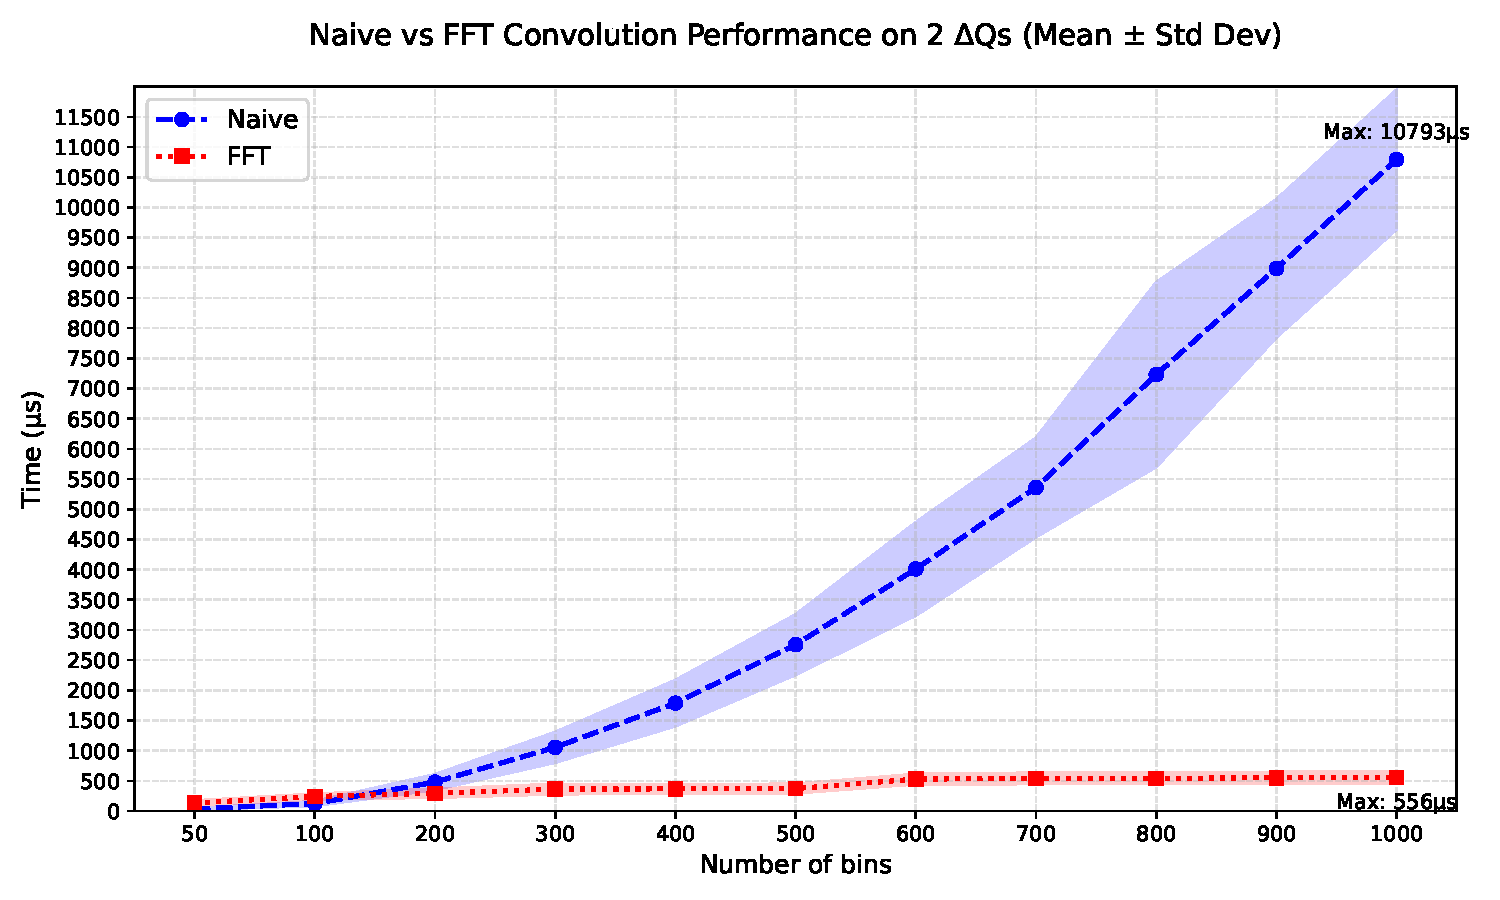
\includegraphics[width=0.85\textwidth]{img/conv_perf.pdf}
        \end{center}
        \caption{Performance comparison of two convolution algorithms}\label{fig:conv_perf}
    \end{figure}

    As expected, the naïve version has a time complexity of $\mathcal{O}(n^2)$ and quickly scales with the number of bins, this is clearly inefficient, as a more precise $\Delta$Q will result in a much slower program.

As for the FFT algorithm, it is slightly slower when the number of bins is lower than 100. This is due to the FFTW3 routine having slightly higher overhead. Moreover, if we look closer at the FFT graph, we can observe slight increases after we surpass powers of 2 (e.g at 600 $>$ 512, 300 $>$ 256 \dots). This is because the algorithm is based on $\Delta$Qs which are zero-padded to the nearest power of 2, this is to make the calculation more accurate.

While we limit the number of bins to 1000 right now, this limit could potentially be increased as the convolution algorithm is very efficient (0.5 ms for 1024 bins).

    \section{$\Delta$Q adapter performance}
    We evaluated the performance of the adapter to measure its impact in a distributed application. We tested the following calls which represent a normal usage of the adapter.
    \begin{itemize}
        \item \texttt{start\_span} $\rightarrow$ \texttt{end\_span}.
        \item \texttt{with\_span} with the following function: \texttt{fun() $\rightarrow$ ok.}
        \item \texttt{start\_span} $\rightarrow$ \texttt{fail\_span}.
    \end{itemize}

    We ran the simulation for 25000 subsequent iterations, the results are shown in \cref{fig:stub_perf}. 

    The overhead is minimal, around 10 microseconds on average to start and end/fail a span. The same cannot be said about with span, the increased overhead is nevertheless due to a function needing to be called inside it for it to record a span.  
    This shows that the adapter can be integrated seamlessly into an application that was instrumented with OpenTelemetry without presenting noticeable overhead.

   \begin{figure}[H]
        \begin{center}
            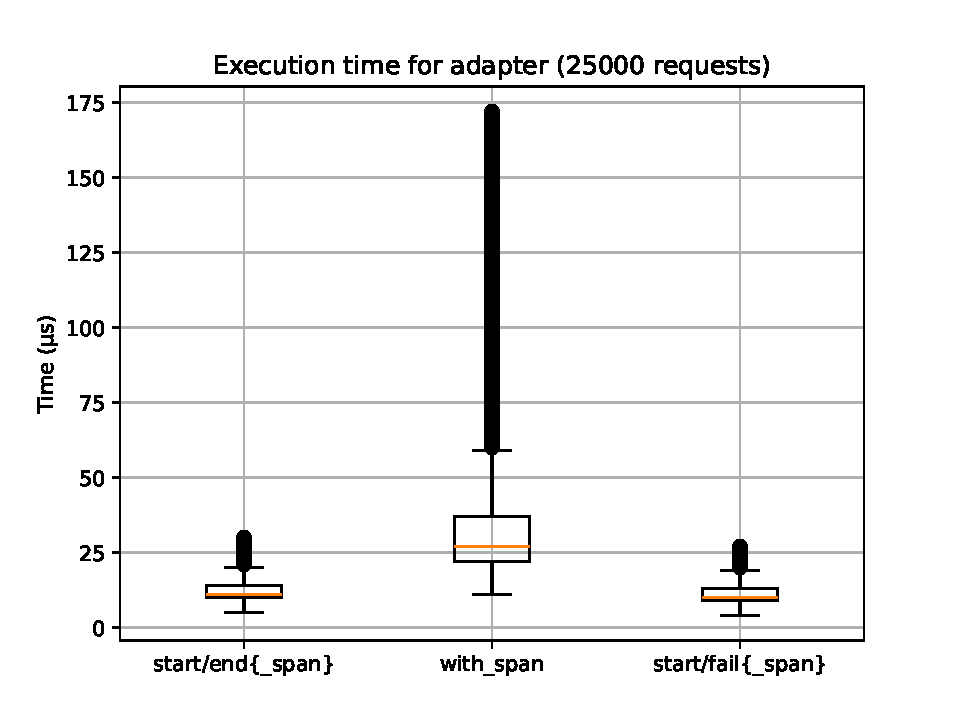
\includegraphics[width=0.7\linewidth]{img/adapter.pdf}
        \end{center}
        \caption{Adapter performance evaluation.}
        \label{fig:stub_perf}
    \end{figure}

 
    \section{GUI plotting performance}
    We evaluated the performance of the GUI plotting routine. We evaluated the routine when plotting the sampling window observed $\Delta$Q and the mean and confidence bounds of the polling window of observed $\Delta$Qs. 
    \begin{figure}[H]
        \begin{center}
            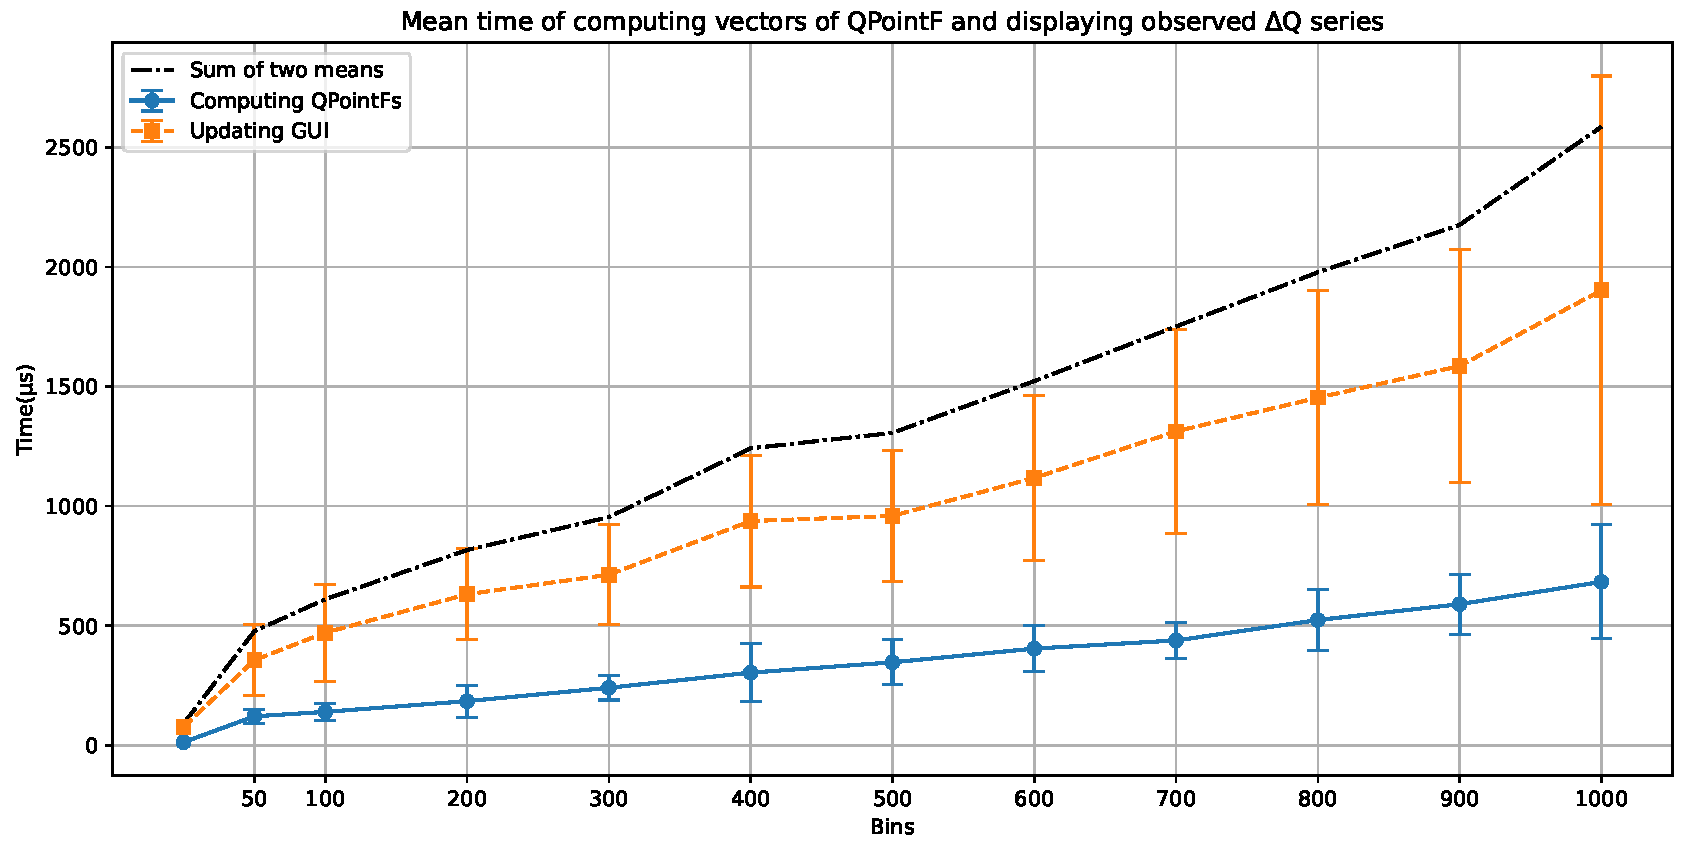
\includegraphics[width = 0.85\textwidth]{img/plots.pdf}
        \end{center}
        \caption{Performance of plotting sampling window and polling window observable $\Delta$Q. \textbf{(Blue, circle)}: QPointF vectors setup performance. \textbf{(Orange, square)}: Plotting performance. \textbf{(Black, dotted)}: Sum of the previous two.}
    \end{figure}
    The procedure for preparing and plotting the observed and calculated $\Delta$Q (along with the confidence bounds) is the same, so we would need to double the results we have to obtain the total time for the plot of a sub-outcome diagram or an operator.
    The routine first prepares vectors of QPointF \cite{qpointf}, representing all the x and y values of the $\Delta$Qs CDF. The vectors are created for the lower bounds, the upper bounds, the mean of the window of $\Delta$Qs and the observed $\Delta$Q.

    Then, once the vectors are prepared, Qt replaces the old points of a series with the new points for every series being plotted.

    The result scales up to almost 2.5 ms for 1000 bins. We believe that these performances are a big bottleneck of the oscilloscope. If we were to plot the calculated $\Delta$Q and its confidence bounds, the time increase would be twofold. If the sampling rate was 100ms and many probes plots were being displayed, some frames would probably be skipped if the number of bins is high. The results we obtained may nevertheless be explained by the specifications of the PC where we ran the tests, namely by the CPU and the GPU (\cref{app:pc_spec}).

